\section{Designing Large-scale Socio-Technical Systems}
\label{sec:design}
% Always give a unique label
% and use \ref{<label>} for cross-references
% and \cite{<label>} for bibliographic references
% use \sectionmark{}
% to alter or adjust the section heading in the running head


%\begin{figure}[h!]
%\begin{center}\footnotesize
%	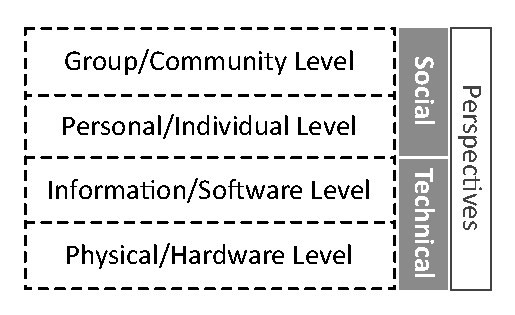
\includegraphics[width=1.0\linewidth]{img/sts_levels.pdf}\\
%	DSO (Distribution System Operators),  SSL (Secure Sockets Layer)
%	\caption{YouPower Platform Overview}\label{fig:platform}
%\end{center}
%\end{figure}

\begin{figure}[t]
\sidecaption[t]
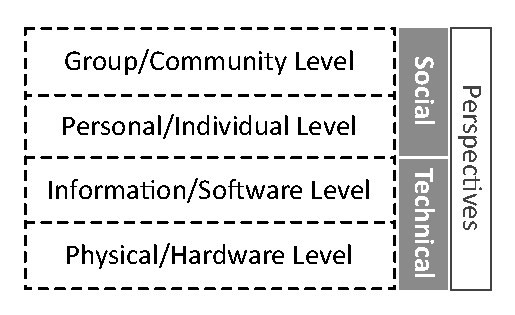
\includegraphics[scale=.5]{img/sts_levels.pdf}
\caption{Levels of STS viewing from different perspectives: the levels are not different systems but overlapping views of the same system \cite{Whitworth2009,Whitworth2013}}
\label{fig:sts_levels} 
\end{figure}

STS are systems arising through encompassing people communicating with people whose interactions are mediated (at least partially) by technology rather than only in the natural world \cite{Whitworth2009}.
The term ``socio-technical'' embodies both a research perspective and a subject matter \cite{Lee2001}. Facing a complex system, researchers from different disciplines often examine the system from their own perspectives. Engineers, for example, see hardware systems, computer scientists see information systems, psychologists see cognitive systems, sociologist see social systems -- all these views are valid \cite{Whitworth2013}. 
Figure~\ref{fig:sts_levels} uses the notion of system levels to illustrate this  difference of perspectives in STS \cite{Whitworth2009,Whitworth2013}. Notably, the levels in Figure~\ref{fig:sts_levels} are not different systems nor partitions of systems, but overlapping views of the same system corresponding to the engineering, computing, psychological and sociological perspectives \cite{Whitworth2009}. The top and bottom of the levels are open-ended, 
as social groups can coalesce into larger entities such as organizations, cities, nations and beyond \cite{Whitworth2009a}, while physics and hardware can be studied in micro, nano and smaller scales. The system boundary and the boundaries of those views are not necessarily clear-cut (hence drawn as dashed lines). An STS view is one that incorporates and meaningfully interconnects all levels of considerations: the upper two levels (Group/Community and Personal/Individual) together being social and the lower two (Information/Software and Physical/Hardware) technical. Each upper level can be seen as   ``arising'' or ``emerging'' from the lower levels. For example, personal cognitions ``emerge'' from information exchanges supported by software, which ``arises'' from hardware \cite{Whitworth2009}. The higher a level of view, the higher its degree of abstraction, and the less deterministic and predictive it becomes.  
% 
With the levels of these different perspectives in mind, the STS view can be articulated as the recognition of three fundamental properties as follows \cite{Sawyer2014}. 
%
%
\begin{description}
\item[\textit{First, the mutual constitution of people and technologies.}] 
This mutual constitution (by the social and the technological) generates complex and dynamic interactions among technological capacities, social norms, histories, situated context, human choices, actions and so on. In STS, social interactions are enabled or supported by technological means. The two adapt to one another, which is referred to as mutual adaptations. 
%
\item[\textit{Second, the contextual embeddedness of the mutuality.}] 
The context of a sociotechnical system is not taken as static or delineable. There are dynamic situational and temporal conditions that influence 
the mutual adaptations throughout the course of design, development, deployment, uses and even retirement phases of systems of interest. 
%
\item[\textit{Third, the importance of collective action.}] 
Collective action refers to the joint pursuit of one or more shared (potentially conflicting) goals by two or more interested parties such as problem owners, shareholders, users  and communities affected (without implying positive or negative outcomes). It shapes and is shaped by both the context and the technological components. 
\end{description}
%
%
Researchers who hold an STS view investigate more than just the technological (sub-)system or just the social (sub-)system or even the two side by side, but also the phenomena that emerge when the two interact \cite{Lee2001}. An ST approach tries to abstain from oversimplifications that seek a single or dominant cause of change, but studies the complexity, dynamic and uncertainty in the networks of institution, people and technological artefacts in the process of technologically involved change \cite{Sawyer2014}. 
%
The levels of perspectives and the three fundamental properties of STS aforementioned help researchers to organize, categorize and allocate their inquiries and knowledge. 

What does an STS view mean to design in particular? The rest of this section discusses the impact of an STS view on (I)~the understanding of design problems, and (II)~the design process and design artefacts.

\runinhead{Understanding the Design Problems or Situation} Designing STS is becoming increasingly challenging partly due to the increasing systems complexity and scale.  
Large-scale STS often are not designed as a whole by one team in one project, but are incrementally ``piece by piece'' transformed and evolved from many generations of ``legacy'' systems. Designers and engineers are therefore faced with ill-structured or wicked problems that do not allow to straightforward determine what systems boundaries to choose, what issues to address and what aspects to consider regarding the design \cite{Bots2007}. 

An STS view by definition advocates a systemic approach towards understanding including but not limited to information acquisition, diagnosis and analysis. Developing an understanding of the design problems or situation entails firstly looking into the roles, responsibilities, powers, interests and requirements of the stakeholders involved \cite{Checkland1981}. As will be discussed later in this section, iterations in a design process deepens this understanding. 
Pragmatically, a designer can start with upper level (more abstract) views and dive into the lower level (less abstract) ones. %, i.e. from group/community level towards physical/hardware level as shown in Figure~\ref{fig:sts_levels}.
At each level, a designer investigates questions such as what are the corresponding goals to achieve (or problems to tackle) \cite{Checkland1981,Waterson2002} and associated requirements to fulfil \cite{Whitworth2009a}, which social/technical elements (or components) are important to each level of views, how do the elements operate/behave individually, how do they interact within and across the levels, and what are the possible outcomes of the interactions and in what context \cite{Baxter2011}. 
%
Table~\ref{tab:questions} provides a set of such questions categorized by the three STS properties and associated to the levels of focus. The questions are by no means exhaustive but serve as examples to orient ways of thinking during design. 
Given the nature of STS, the answers to many of such questions are context specific, influenced by situational and temporal conditions \cite{Baxter2011,Norman2015}. This means the contextual information associated with the answers also need to be well studied and documented. 
% 
\begin{table}
\caption{Examples of questions to investigate categorized by STS properties and associated to levels of focus}
\label{tab:questions}       % Give a unique label
%
% Follow this input for your own table layout
%
\begin{tabular}{>{\raggedright}p{2cm}>{\raggedright}p{2.1cm}p{7.5cm}}
\hline\noalign{\smallskip}
\textbf{Properties}  & \textbf{Levels of Focus} &   \textbf{Examples of Questions to Investigate} \\
\noalign{\smallskip}\svhline\noalign{\smallskip}
Mutual constitution & All  & Which elements (or components) are important at each level? $^a$  How do the elements behave and interact?\\
 &  & What are the possible outcomes of the interactios?\\
 &  & What are the goals, constrains and requirements, if any, of the elements?\\ \hline\noalign{\smallskip}
Contextual embeddedness &   Group/ community & What are the situational and temporal conditions where the behaviours and interactions take place? \\
 & Personal/ individual  & What are the influences of  the situational and temporal conditions on the outcomes of the behaviours and interactions?\\
 &  & How those situational conditions may change over time?\\ \hline\noalign{\smallskip}
Collective action   & Group/ community & What are the community (or institutional) goals, constrains and requirements?\\
   &  Personal/ individual  & How are the community (or institutional) goals, constrains and requirements aligned with the individual goals, constrains and requirements? \\
   & & What is the group and individual attitude towards the community (or institutional) goals or collective action? \\ \hline\noalign{\smallskip}
General $^b$ & All  & What is the level of resolution to use when describing and analysing the system? \\
& & What is the set of values that underpin the design thinking about the system? \\
& & What are the criteria and metric of evaluating whether and to what extent the desired goals are achieved and maintained? \\
\noalign{\smallskip}\hline\noalign{\smallskip}
\end{tabular}
$^a$ Elements can also be categorized by weighted scale, e.g. from \textit{important} (must be included in the study), to \textit{can be relevant} (can be included in the study), to \textit{not relevant} (can be excluded from the study).\\
$^b$ It concerns all three properties above. 
\end{table}
%
%
\begin{figure}[b!]
\centering
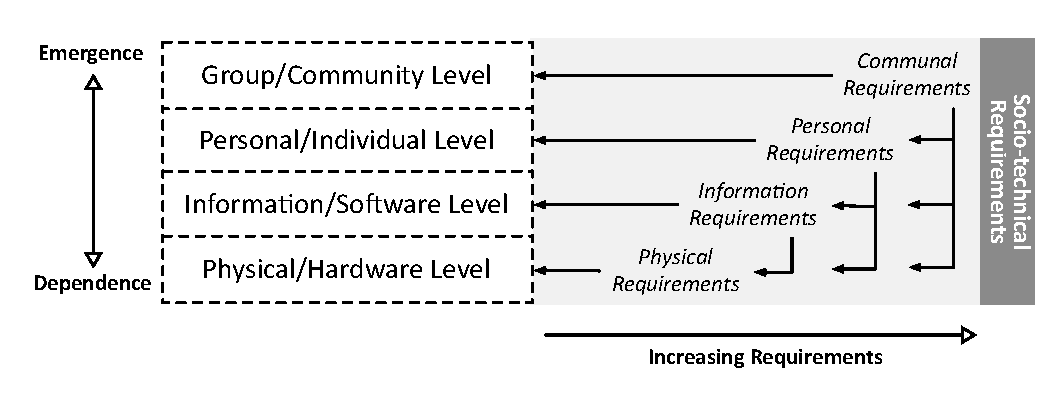
\includegraphics[width=.82\linewidth]{img/sts_requirements.pdf}
\caption{Levels of socio-technical requirements \cite{Whitworth2009a}}
\label{fig:sts_requirements} 
\end{figure}
% 
%
In an ST approach, social requirements must become part of the technical design \cite{Whitworth2014}. Figure~\ref{fig:sts_requirements} illustrates the relation of requirements at different levels \cite{Whitworth2009a}. Each level unveils requirements that cumulate level by level. The requirements at one level affect not only that level but all those below it \cite{Whitworth2009a}. For example, a communal requirement may add new requirements at the personal level which in turn affects software and hardware requirements. When a technical design fails to fulfil requirements derived from the personal or social level, there is a deficit  between  what  society  needs  and  what technology does -- this is when a ``ST  gap''  emerges \cite{Whitworth2014}. 


As mentioned earlier, large-scale STS are often``systems of evolution'' rather than ``systems of revolution'' \cite{Baxter2011,Norman2015}. Significant changes in a system should be accompanied by a well designed and managed change process where feedback is returned for analysis and adaptation \cite{Baxter2011}. For this, a good understanding of the existing system and work/operation processes is necessary to design and plan the change process. Many core difficulties in complex projects stem from implementation of the design in the real world \cite{Norman2015}. Designers therefore need to address the possible impediments to implementation (and change process) already from the beginning, and they must play an active role in implementation, and develop solutions through small incremental steps \cite{Norman2015}.

\runinhead{Design Process and Design Artefacts} The design process of STS is often conceived and implemented as a participatory decision-making process where problem owners, shareholders, users, developers and other stakeholders are actively involved to represent their interests and negotiate agreements. 
Designers should be working \textit{in} the context of an STS as an insider, not outside of the system as a bystander, with the intention of changing or improving some part of that system \cite{Bots2007}. 

The evolutionary nature of STS means that what matters more in the design is the design process itself rather than the ``final status'' of the system \cite{Shin2014}. When an STS keeps evolving and exhibits emergent behaviour \cite{Nikolic2009}, any designed ``final status'' soon becomes a transitional state. An important goal of a design process is to make the design relevant to the evolving context where the technology is utilized \cite{Shin2014}. This is not a pure technological inquiry but an ST one that demands human-centred design, progressing by iteration and ``muddling through'' \cite{Norman2015}. 

The interdisciplinary nature of STS calls for interdisciplinary teams. Although this need has been widely accepted, working in an interdisciplinary team remains a persisting challenge. 
It is group work of the most challenging sort, especially when those involved are in fields far apart intellectually as well as physically \cite{Brewer1999}. 
Despite efforts at creating teams across disciplines in the design process, interdisciplinary integration is often poor and disciplinary borders have been largely maintained \cite{Baxter2011}. Some common issues include \cite{Baxter2011,Brewer1999,Norman2015}: (1) difficulties concerning the logistics of group interactions at management level; (2) failures in understanding and communication due to methodological, disciplinary, language, cultural and value differences; (3) personal challenges related to gaining trust and respect of others working in different disciplines, and (4) institutional impediments related to incentives and priorities given to disciplinary versus interdisciplinary work.
% 
One discipline has to understand (at least at an conceptual level) and appreciate what the other disciplines can do in order to ask them to deliver something that assists the analysis and design during the development process \cite{Baxter2011}. 

% there needs to be agreement about the social and technical elements of the systems that need to be jointly considered, if possible optimised. this particularly applies to the development team in order to make sure that they focus on the appropriate social and technical aspects, and study how their interdependence and interaction 

The design artefacts can be aligned to achieve specific goals or effects across all four levels of views (shown in Figure~\ref{fig:sts_levels}) through which designers wish to intervene in STS. They can be, for example, hardware, software artefacts, a new idea of human-computer interaction design, rules for behaviour, policies, social programs, and any combination of them. Good solutions are often balanced ``satisficing'' solutions between different requirements that will be acceptable to and used by end users as well as delivering the expected benefits to stakeholders \cite{Baxter2011,Norman2015}. 
As mentioned earlier, designers should not stop at the design stage but play an active role in implementation, developing ``evolving'' contextual solutions through iteration \cite{Norman2015}. Acontextual and detemporalized general solutions are actually self-limiting \cite{Sawyer2014}. 
% 
In addition, the solutions should be accompanied by a thoughtful change process that is concerned with, among others, sensitising stakeholders for awareness and constructive engagement taking into account social and organizational issues \cite{Baxter2011}.


%\begin{svgraybox}
%
%---system design does not take into account human psychology
%---human tendency to want simple answers, docompose systems and straightforward linear causality 
%
%focus on situating work and seek to examine all contextual factors, this types of inquiry attempt to construct a holistic view of context: one that does not diminish or remove contextual elements, even those with limited influence. 
%
%\end{svgraybox}


